There are a lot of companies providing services that do real-time communications out on the market today. First we will take a look at similar technologies\cite{lopez_fernandez_catalysing_2013} that is in direct competition with \gls{wrtc}, in addition we will look at businesses that are looking to incorporate real-time communications into their existing services.

\subsection{Real-time communications}
For doing real-time communications the biggest vendors are Cisco, Polycom, and Microsoft as seen in figure \ref{fig:room-based-videoconferencing} and figure \ref{fig:desktop-videoconferencing}.

\begin{figure}[here]
\centerline{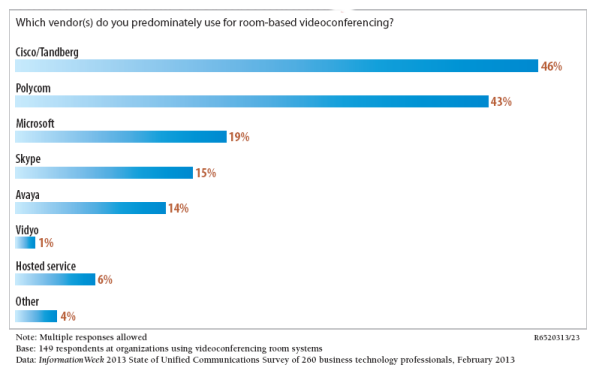
\includegraphics[scale=0.75]{room-based-videoconferencing.png}}
\label{fig:room-based-videoconferencing}
\caption{Vendors used for room-based videoconferencing}
\end{figure}

\begin{figure}[here]
\centerline{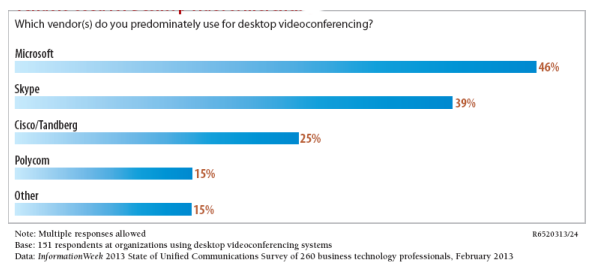
\includegraphics[scale=0.75]{desktop-videoconferencing.png}}
\caption{Vendors used for desktop videoconferencing}
\label{fig:desktop-videoconferencing}
\end{figure}

Cisco and Polycom are clearly the big winner with their room-based videoconferencing systems, but Microsoft is winning the desktop market with their Lync and Skype applications. Skype utilizes a peer-to-peer model by leveraging all of the available resources in a network, this is probably why they can manage free communications, as using centralized resources are very costly. Skype has very successfully developed an audio/video communications platform with their technology, however the same type of model is used by \gls{wrtc} to allow for efficient use of resources.

\subsection{WebRTC for service markets}
Customer-services depend heavily on communications, but these services have mostly been concentrated around the traditional telephone and more recently browser based chat messaging. Now there is a trend to incorporate live chat with video as well in this market\cite{amazon_mayday}. It's all about having a personal experience and engaging with the customer. Especially e-commerce sites are looking to integrate \gls{wrtc} as part of their customer service experience. Emerging companies take advantage of these needs creating services that simplify the integration of \gls{wrtc}. Even the companies in the figures above have said to be working on how they can use \gls{wrtc} in their own systems\cite{polycom-webrtc}. Ericsson was the first to deliver an interworking gateway\cite{ericsson-gateway} much like the one I am trying to model in this thesis. However, their solution is for commercial use and closed for the public eye.

\subsection*{Summary}
Enterprise communication vendors have made significant investments to build their services, and with the introduction of \gls{wrtc} these companies are threatened by upcoming competing enterprises. But they are not naive, most of them are looking into how they themselves can use the \gls{wrtc} technology. It's going to be exciting to see if the market shifts in favor of WebRTC over traditional enterprise systems.